\documentclass[12pt]{article}

\usepackage[italian]{babel}
\usepackage[T1]{fontenc}
\usepackage{charter}
\usepackage{bookmark}
\usepackage{geometry}
\usepackage{graphicx}
\usepackage{float}
\usepackage{extsizes}
\usepackage{blindtext}
\usepackage{wrapfig}
\usepackage{ragged2e}
\usepackage{xcolor}
\usepackage{subcaption}
\usepackage{keyval}
\usepackage[format=plain, textfont=sl, font=footnotesize]{caption}
\usepackage{hyperref}

\geometry{
 a4paper,
 total={170mm,262mm},
 left=20mm,
 top=20mm,
 }
\graphicspath{ {res/} }
\hypersetup{
    colorlinks = false,
    pdftitle = {Smart Room Report},
    pdfpagemode=FullScreen,
}
\captionsetup[figure]{labelformat=empty, justification=centering}
\setlength\intextsep{0pt}
\def\code#1{\texttt{#1}}

\title{Smart Room}
\author{Marco Antolini, Luca Pasini, Lorenzo Tosi, Andrea Zavatta}

\begin{document}

\topskip0pt
\begin{center}
    \vspace*{\fill}
    \Huge{Relazione progetto Smart Room \code{-} IoT} \\
    \vspace*{\fill}
    \Large\textsl{Marco Antolini, Luca Pasini, Lorenzo Tosi, Andrea Zavatta} \\
    \vskip 1cm
    \large\textsl{marco.antolini6@studio.unibo.it, luca.pasini9@studio.unibo.it, lorenzo.tosi10@studio.unibo.it, andrea.zavatta3@studio.unibo.it}
    \vspace*{\fill}
\end{center}

\newpage

\tableofcontents
\newpage

% -------------------- Requisiti --------------------

\section{Requisiti}

Desideriamo realizzare un sistema IoT che implementi una versione semplificata di una stanza intelligente, finalizzata a monitorare e controllare lo stato di una stanza in un campus.\newline
\textit{\code{1.}} \textbf{Room Sensor Board} (esp): Sistema incorporato per monitorare lo stato della stanza tramite sensori. Interagisce con il Room Service tramite MQTT o HTTP.\newline
\textit{\code{2.}} \textbf{Room Service} (backend \code{-} pc): Funziona come unità principale per la gestione della stanza. Comunica tramite seriale con il Controller, tramite MQTT con la Room Sensor Board e tramite HTTP con la Dashboard.\newline
\textit{\code{3.}} \textbf{Room Controller} (Arduino): Sistema incorporato che controlla la luce e le serrande. Comunica tramite seriale con il Room Service e tramite Bluetooth con la Room App. Deve implementare la logica di controllo tramite macchine a stati finiti (sincrone o asincrone).\newline
\textit{\code{4.}} \textbf{Room App} (Android \code{-} smartphone): App mobile per il controllo manuale delle luci e delle serrande. Comunica con il Controller tramite Bluetooth (o tramite seriale in caso di emulatore Android).\newline
\textit{\code{5.}} \textbf{Room Dashboard} (Frontend/web app su PC o tramite sockets): Interfaccia per visualizzare e tracciare lo stato della stanza. Interagisce con il Room Service.\newline
Il sistema Smart Room controlla l'illuminazione e le serrande secondo la seguente politica:\newline
- Se nessuno è nella stanza, la luce è spenta.\newline
- Se qualcuno entra in una stanza buia, la luce si accende.\newline
- Le serrande si sollevano completamente automaticamente alla prima entrata a partire dalle 8:00.\newline
- Le serrande si abbassano completamente alle 19:00 se sono sollevate e nessuno è in stanza, o non appena chi è ancora in stanza alle 19:00 lascia.\newline
Attraverso l'app mobile, l'utente può:\newline
- Accendere/spegnere la luce.\newline
- Sollevare/abbassare le serrande in modo parziale (0\code{-}100\%).\newline
- Attraverso la dashboard, il responsabile della stanza può:\newline
- Monitorare lo stato della stanza.\newline
- Controllare completamente la luce e le serrande.\newline
- Si presume che la stanza sia accessibile dalle 8:00 alle 19:00.\newline
Ulteriori dettagli:\newline
- La Room Sensor Board deve accendere il LED quando qualcuno è in stanza e spegnerlo quando nessuno è presente.\newline
- Il Controller controlla/simula le serrande con un servomotore. 0° rappresenta le serrande completamente sollevate, 180° completamente abbassate.
\vskip 0.3cm
\begin{figure}[H]
    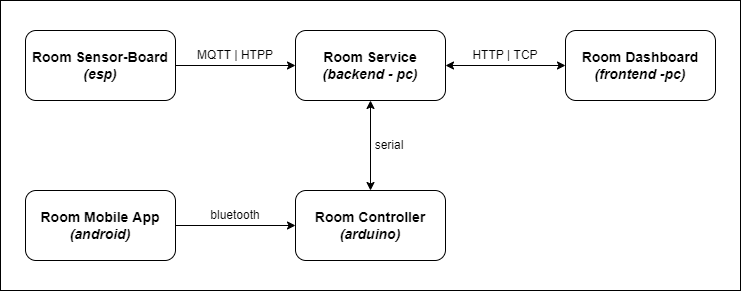
\includegraphics[width=17cm]{application-schema.png}
    \centering
    \caption{Schema funzionamento applicazione}
    \centering
\end{figure}
\newpage

% -------------------- Room Sensor Board --------------------

\section{Room Sensor Board}

\subsection{Descrizione}
La "Room Sensor Board" consiste in un sistema embedded che ha il compito di monitorare lo stato della stanza e i suoi cambiamenti. Vengono utilizzati due sensori: il PIR e un fotoresistore. Il PIR rileva la presenza di una persona nella stanza e il fotoresistore ne monitora il livello di luce presente. Nel caso in cui il PIR rilevi una presenza, allora accenderà la luce, rappresentata da un led. Il dispositivo utilizzato per supportare queste funzioni e sensori è un esp32, un SoC con modulo Wi-Fi e Bluetooth integrati; interagisce con il Room Service attraverso il protocollo MQTT.

\subsection{Architettura}
In questo modulo è stato implementato il funzionamento degli attuatori e dei sensori che costituivano il sistema embedded in questione. Molto importante è quindi l'esp32, i cui compiti sono: comunicare attraverso il Wi-Fi e gestire il funzionamento dei sensori. Il primo compito viene svolto in 2 momenti diversi: inizialmente il dispositivo si connette ad una rete Wi-Fi e, una volta che la connessione è stata stabilita, inizia la vera e propria comunicazione, gestita attraverso un \textbf{Task} chiamato \code{Execute} ed eseguita grazie ad uno \textbf{Scheduler}. Questo task ha anche il compito di gestire il funzionamento dei sensori.\newline
\begin{figure}[H]
    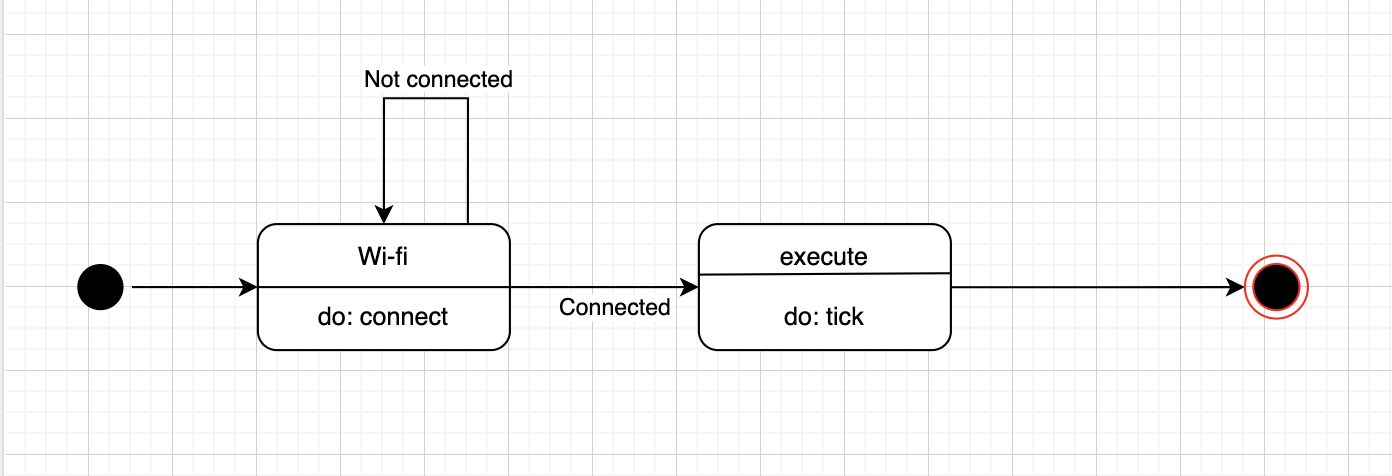
\includegraphics[width=17cm]{esp-schema.png}
    \centering
    \caption{Schema funzionamento task \code{Execute}}
    \centering
\end{figure}
\newpage

% -------------------- Room Controller --------------------

\section{Room Controller}

\subsection{Descrizione}
Il "Room Controller" consiste in un sistema embedded che ha il compito di gestire il funzionamento delle serrande e della luce della stanza.\newline
Questo sistema è composto da un led, un modulo bluetooth e un servo motore. Il led simula la luce della stanza, il servo motore le serrande e il modulo bluetooth viene utilizzato per ricevere comandi da un'applicazione mobile. Il dispositivo hardware usato è Arduino.\newline
Questa sottoparte è il core di tutto il sistema: deve essere sempre aggiornata riguardo lo stato della stanza (proprio come il Room Service). Infatti, lo stato può dipendere da ciò che viene registrato dalla Sensor Board, dall’applicazione web che comunica con il sistema attraverso la rete (Room Dashboard) oppure da un'applicazione mobile (Room App). È quindi necessario che tra il Room Controller e il Room Service sia presente una continua comunicazione bilaterale (implementata mediante comunicazione seriale) che mantiene aggiornate e connesse entrambi le parti.

\subsection{Architettura}
Il Room Controller è stato pensato come una FSM sincrona. La logica alla base è suddivisa in \textbf{Task} che vengono eseguiti grazie ad uno \textbf{Scheduler}.\newline
Il task principale è la \code{SmartRoom}: questo gestisce il comportamento di tutte le componenti della stanza. Ogni volta che è presente un messaggio, proveniente dalla comunicazione seriale o bluetooth, questo viene ricevuto e i suoi parametri utilizzati per aggiornare le componenti interessate. Questo task fa uso di un modulo chiamato \code{MsgService} che gestisce la ricezione di dati e l'invio di informazioni necessarie alla Room Service in modo tale che quest'ultima sia sempre aggiornata. Lo scambio di dati avviene attraverso un unico formato: JSON.\@ Questo modulo è anche in grado di comunicare con l'applicazione mobile in quanto gestisce anche le comunicazioni bluetooth.\newline
\begin{figure}[H]
    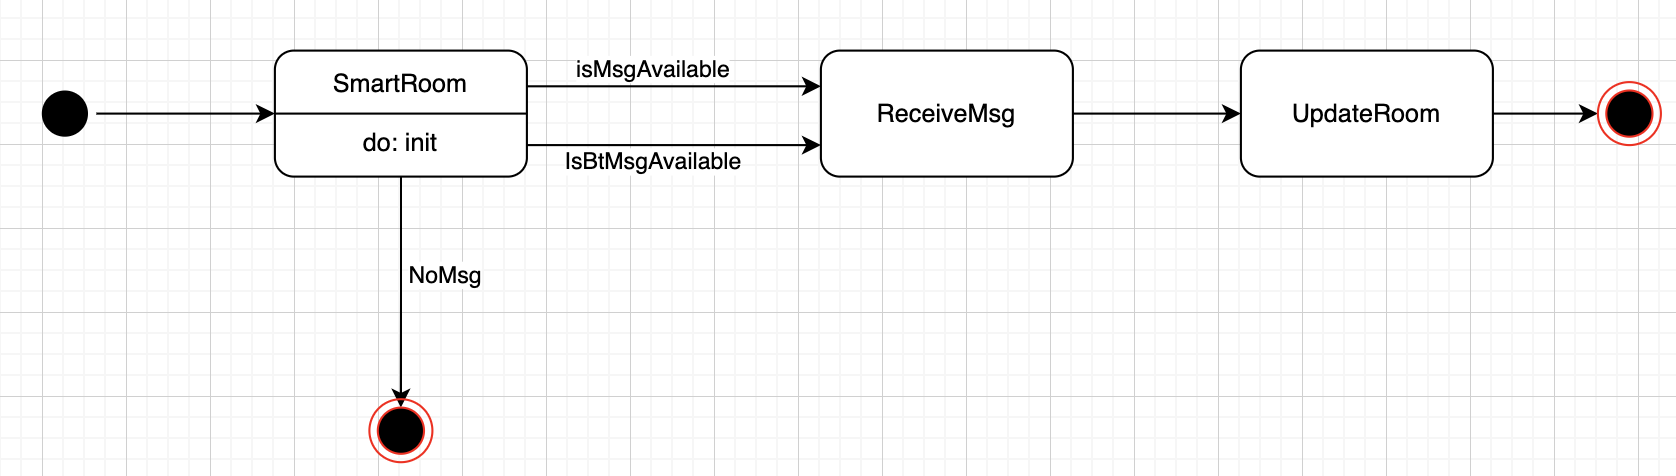
\includegraphics[width=17cm]{arduino-schema.png}
    \centering
    \caption{Schema funzionamento task \code{SmartRoom}}
    \centering
\end{figure}
\newpage

% -------------------- Room Service --------------------

\section{Room Service}

\subsection{Descrizione}
Il Room Service consiste in un file Python che funge da tramite fra le varie parti dell'applicazione. Nello script vengono usati due moduli principali: \textbf{MQTT} per ricevere messaggi dal Room Sensor Board e \textbf{Requests} per la comunicazione tramite richieste HTTP con la Room Dashboard. Inoltre viene utilizzato il modulo \textbf{Serial} per lo scambio di messaggi con il Room Controller.

\subsection{Architettura}
Prima di tutto lo script assegna i valori iniziali per gli stati della stanza (luci e serrande), successivamente viene creato un client MQTT e viene stabilita una connessione con il broker che procederà a notificare lo script quando viene ricevuto un nuovo messaggio sul canale a cui si è iscritto il client.\newline
Lo script poi funziona tramite un loop principale che verifica se sono stati aggiornati i parametri da parte della Room Dashboard per poi informare il Room Controller tramite il seriale. Quando lo script riceve un messaggio dalla Room Sensor Board, prima aggiorna i propri parametri interni poi manda un messaggio alla Room Dashboard e al Room Controller.\newline
\begin{figure}[H]
    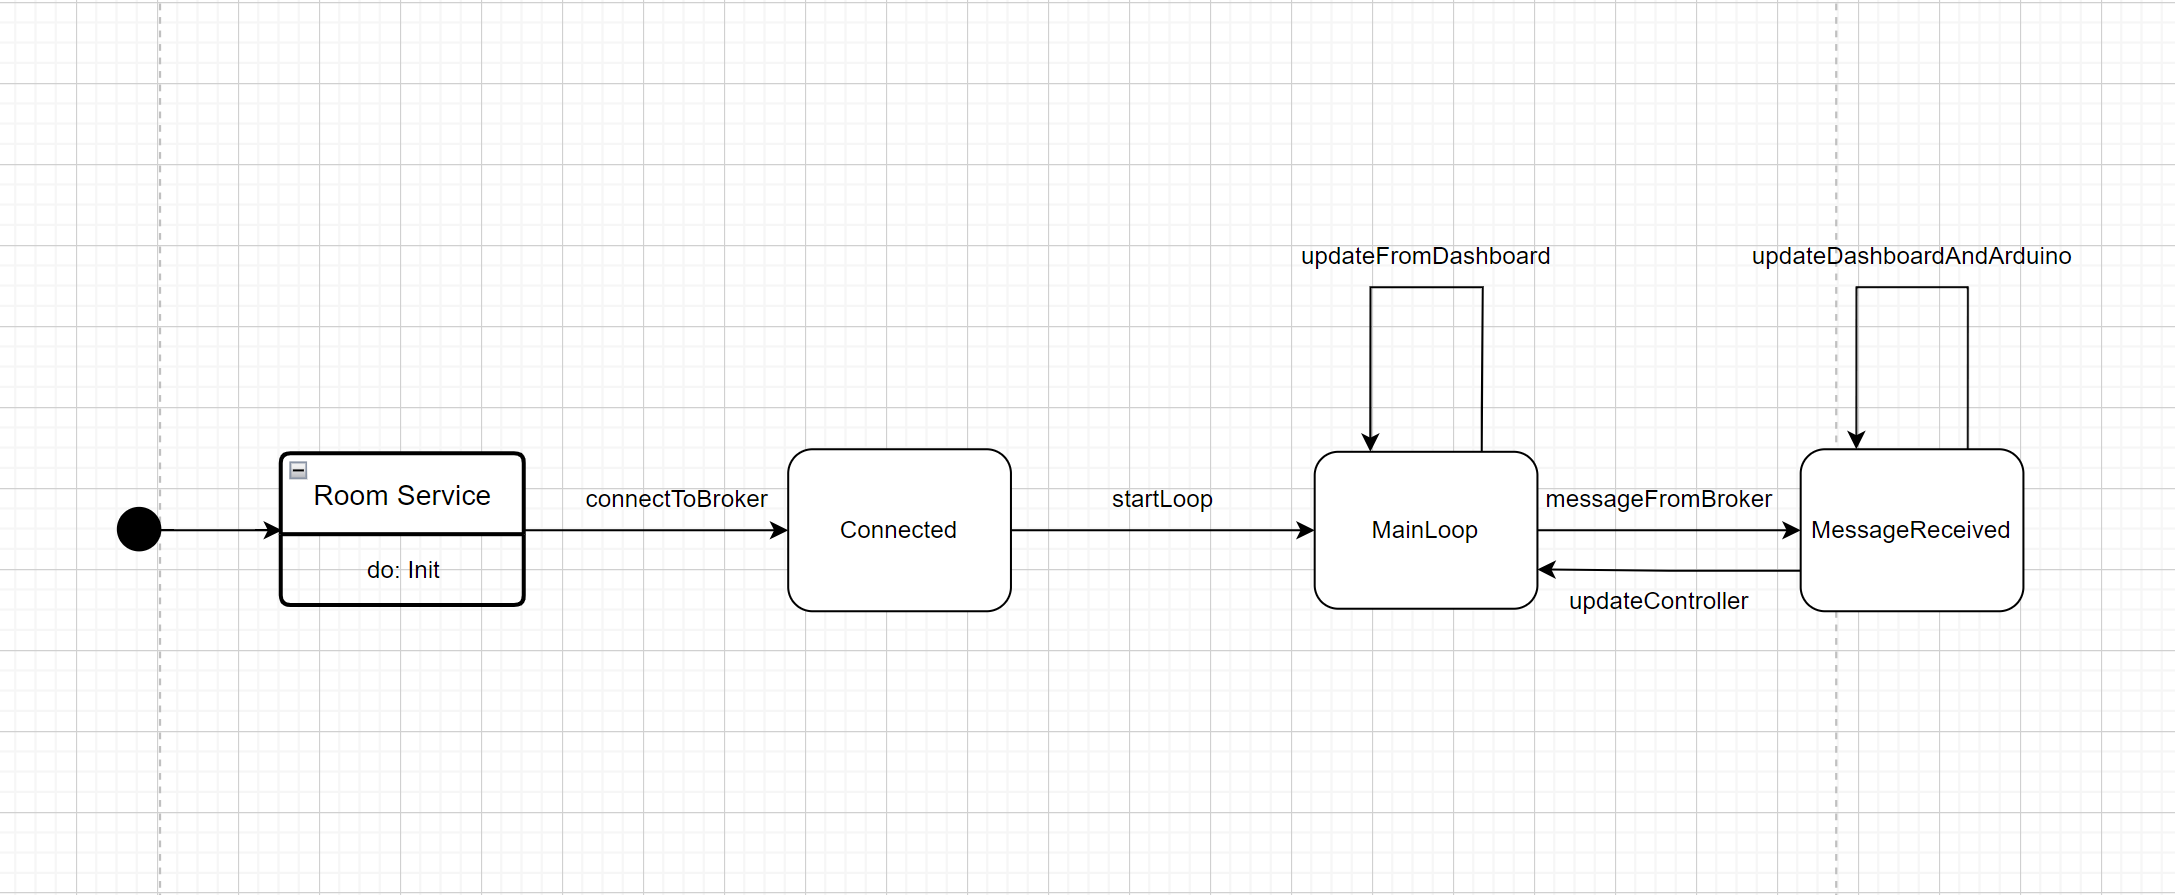
\includegraphics[width=17cm]{room-service.png}
    \centering
    \caption{Schema funzionamento \code{Room Service}}
    \centering
\end{figure}


\newpage

% -------------------- Room Dashboard --------------------

\section{Room Dashboard}

La Room Dashboard è un'applicazione web hostata su localhost grazie al servizio di web server Xampp che comunica tramite richieste HTTP con il Room Service per interagire con i componenti hardware.

\subsection{Software}
Come introdotto in precedenza la dashboard utilizza le richieste HTTP per comunicare con il Room Service in python che permette di scambiare informazioni e comandi in tempo reale con l'hardware.\newline
Tutti i logs delle ultime 24 ore vengono salvati (e aggiornati dinamicamente) sul file \code{logs.json}.\newline
Il file \code{room-dashboard-history.js} deve semplicemente accedere ai logs quindi fa una richiesta di tipo \code{GET} al file JSON ogni volta che la pagina viene aggiornata.\newline
Il file \code{room-dashboard-window.js} deve invece sia fare una richiesta di tipo \code{GET} al file JSON per ottenere i dati aggiornati, sia gestire i comandi provenienti dalla dashboard e farli arrivare all'hardware. Ciò avviene tramite una richiesta \code{POST} al file \code{room-dashboard-history.php} (che tra le altre cose controlla i dati e li filtra per fare in modo che vengano salvati solo quelli delle ultime 24 ore) il quale scrive i dati sul file dei logs.\newline
Dall'altro lato dell'applicazione c'è il Room Service sviluppato in Python che legge i dati dal file dei logs per passarli all'hardware e scrive i cambiamenti hardware sempre sul file JSON.\@ La lettura avviene tramite una richiesta \code{GET} al file \code{room-dashboard-window.php} che a sua volta fa una richiesta di tipo \code{GET} al file JSON.\@ La scrittura invece avviene ugualmente alla controparte della dashboard quindi tramite una richiesta \code{POST} al file \code{room-dashboard-history.php} che successivamente scrive i dati sul file dei logs.
\begin{figure}[H]
    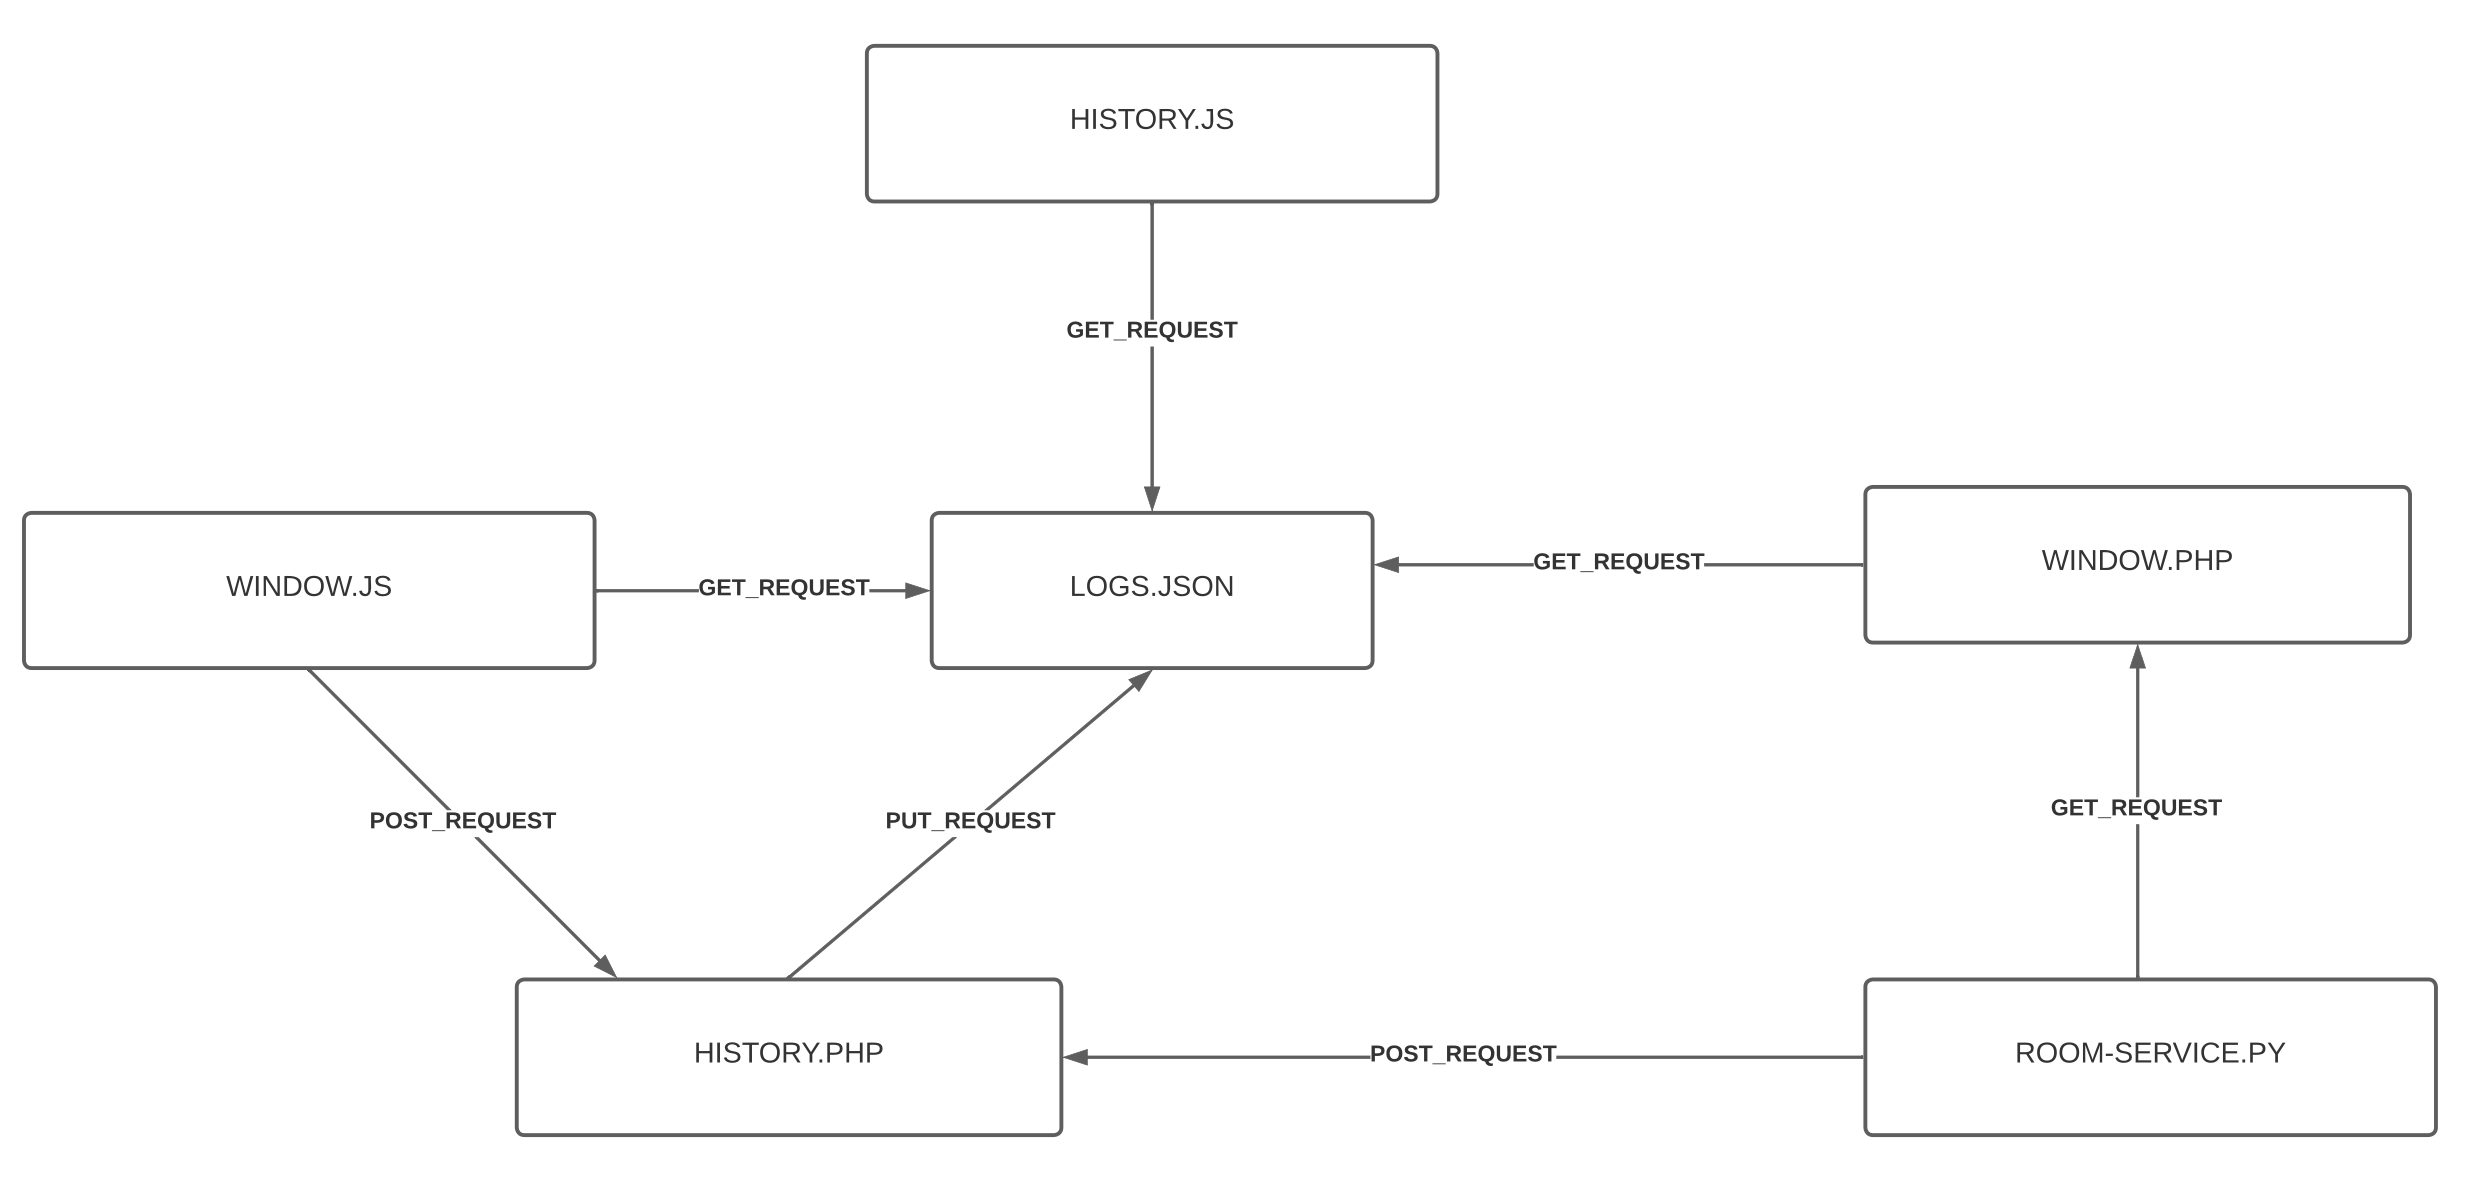
\includegraphics[width=17cm]{dashboard-requests-schema.png}
    \centering
    \caption{Schema funzionamento richieste}
    \centering
\end{figure}

\subsection{Interfaccia}
La dashboard comprende due pagine:
\newline
- Window: mostra lo stato attuale delle serrande e della luce all'interno della stanza e permette anche di modificarli;
\newline
- History: mostra dati relativi all'attività delle serrande e della luce.

\subsubsection{Window}
Nella Window è visibile un orologio che mostra l'orario attuale e lo sfondo del sito cambia dinamicamente in base al fatto che sia giorno o notte. È presente l'immagine di una luce che rispecchia lo stato della luce nella stanza e che è possibile cliccare per accendere e spegnere la luce. Accade lo stesso per le serrande, per cui è presente uno slider tramite il quale è possibile controllare l'apertura totale o parziale delle serrande della stanza.\\
\begin{figure}[H]
    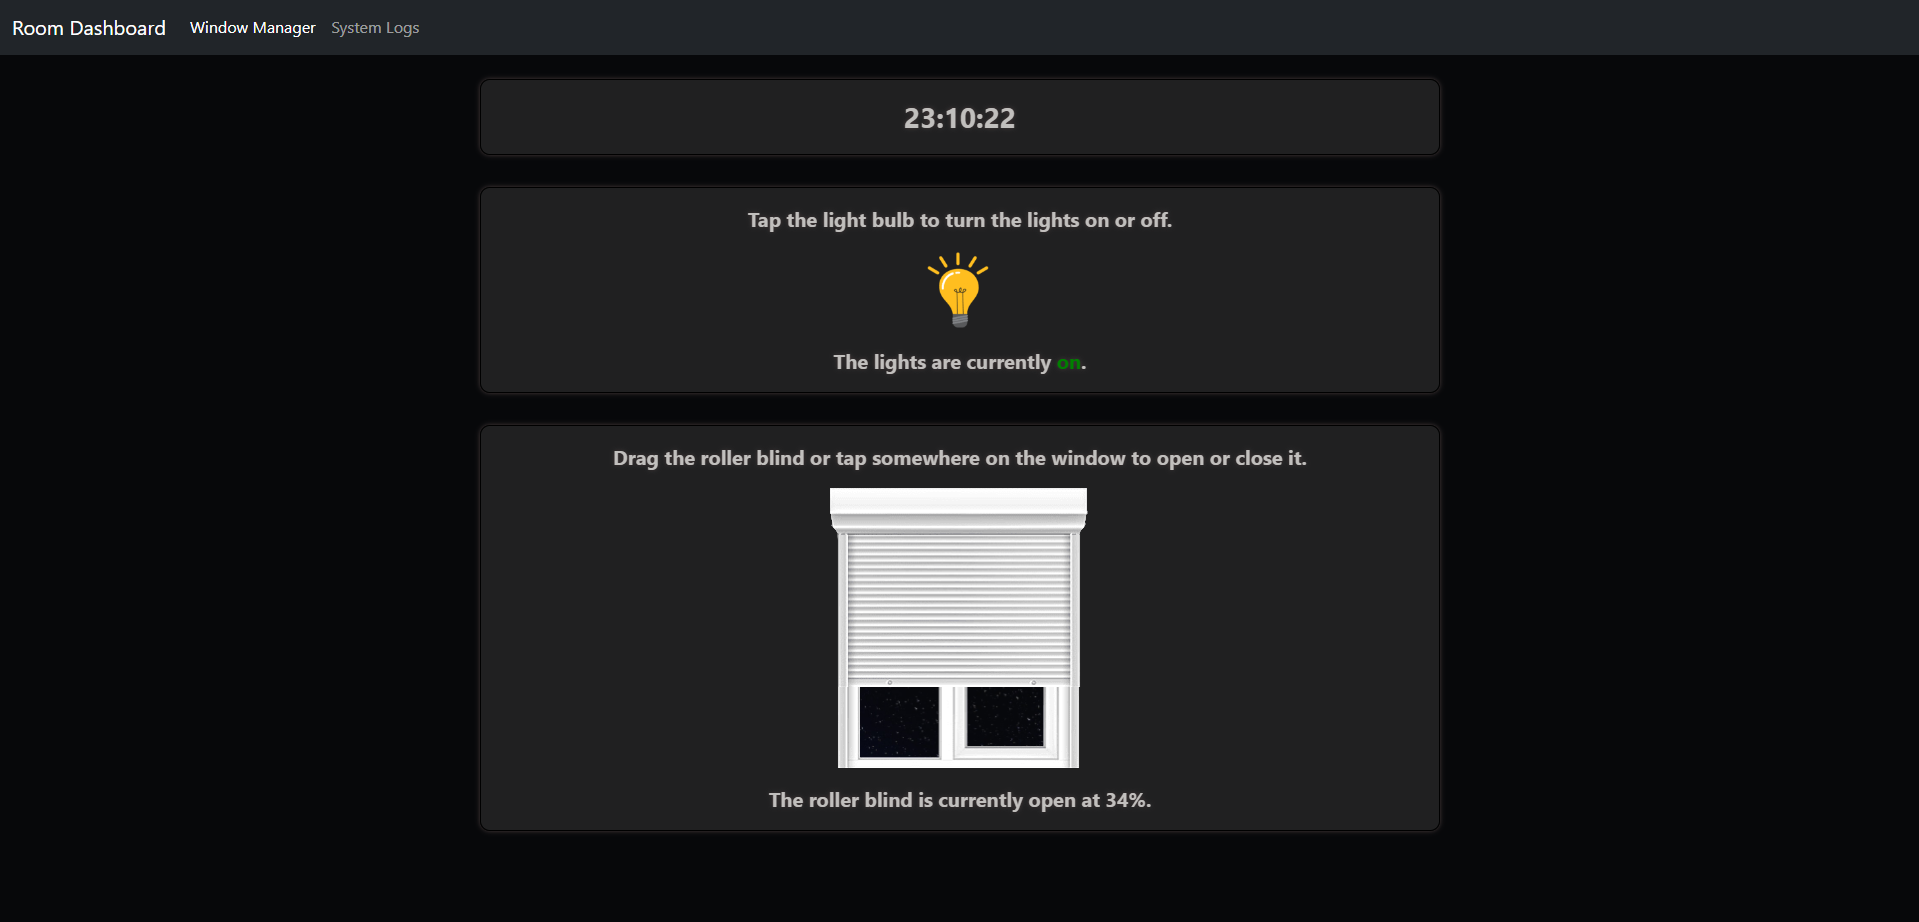
\includegraphics[width=17cm]{dashboard-window.png}
\end{figure}

\subsubsection{History}
Nella History sono presenti due logs che mostrano i momenti (con gli orari riportati in formato HH:mm:SS) in cui la luce è stata spenta o accesa (quindi rispettivamente con le diciture On o Off) e in cui la tapparella è stata aperta o chiusa (riportando la percentuale di apertura rilevata alla fine del movimento).\newline
Inoltre è presente un grafico a torta che mostra l'utilizzo della luce con due fette che raffigurano il tempo in cui è stata accesa e il tempo in cui è stata spenta e le relative percentuali.\newline
Tutti i dati riportati in questa pagina sono relativi alle ultime 24 ore.\\
\begin{figure}[H]
    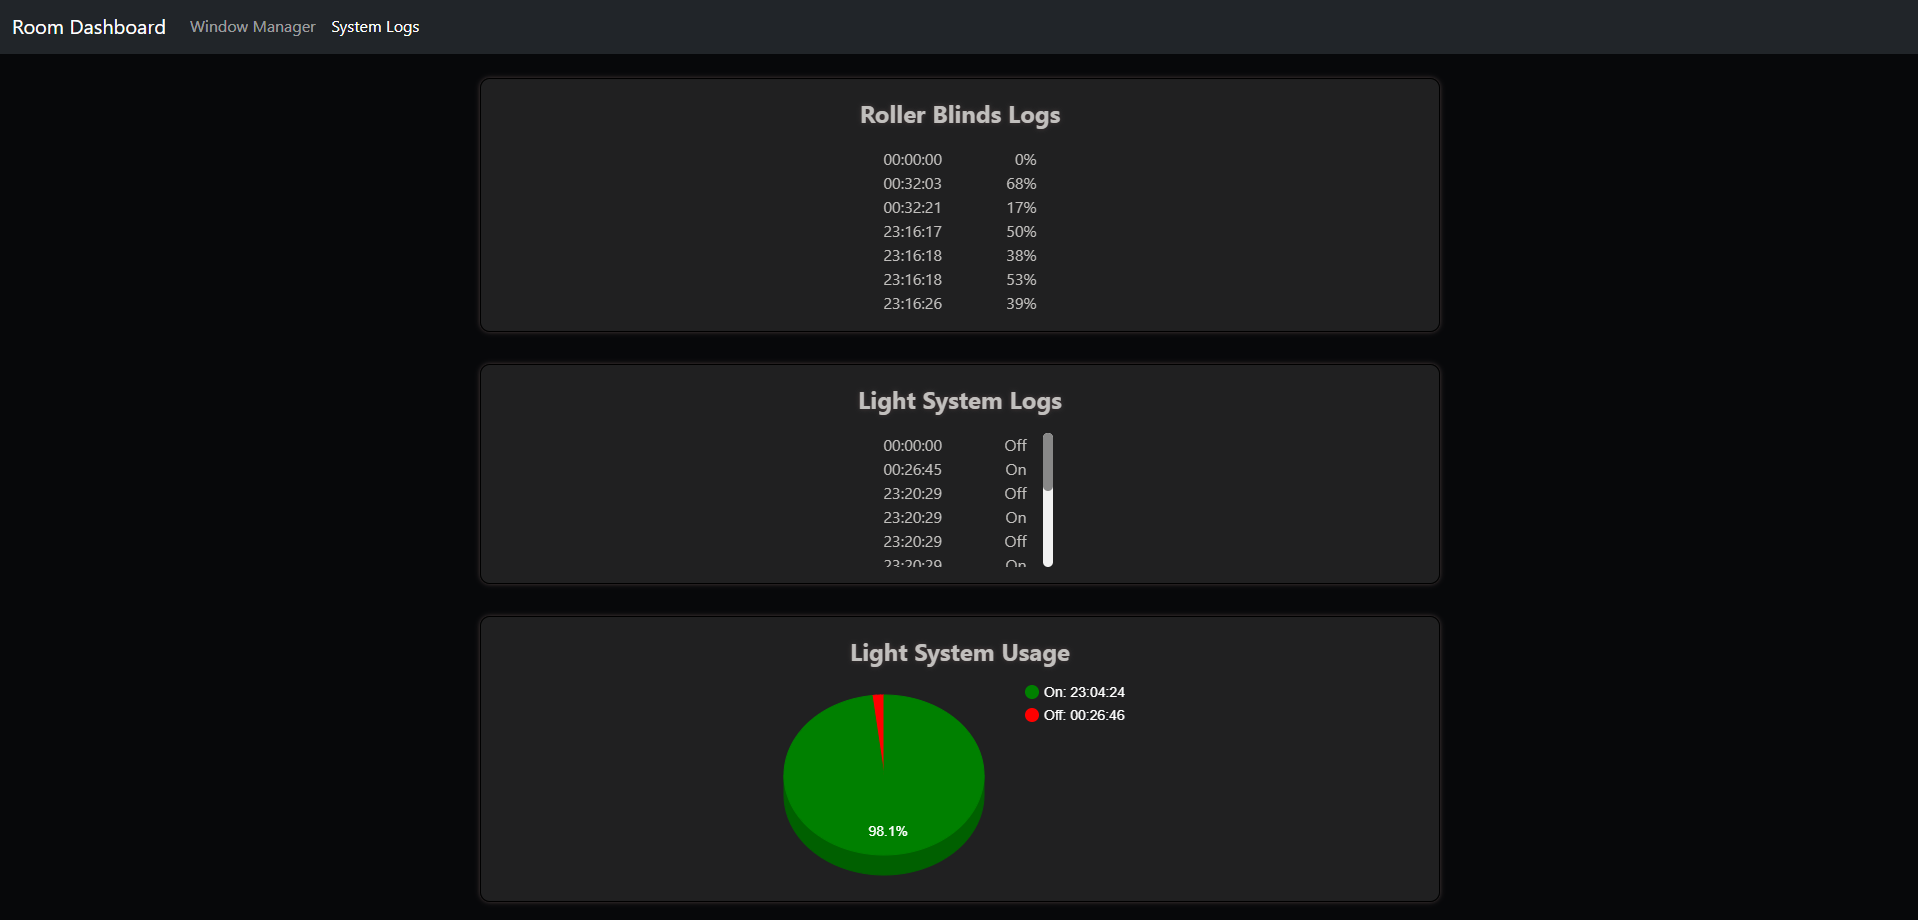
\includegraphics[width=17cm]{dashboard-hisotry.png}
\end{figure}
\newpage

% -------------------- Room App --------------------

\section{Room App}

\subsection{Descrizione}
Per la creazione dell’applicazione è stato seguito il codice fornito a lezione dal Professor Burattini.\\
L’applicazione ha una funzionalità di ricerca dei dispositivi Bluetooth vicini allo smartphone che permette di trovare quello utilizzato da Arduino. L'applicazione effettua dunque un’operazione di pairing. Una volta che i dispositivi sono connessi, all’utente si presenta un’interfaccia con un bottone ed uno slider. Il bottone permette di accendere e spegnere la luce, cambiando colore dal verde (accesa) al rosso (spenta), mentre lo slider serve per regolare l'apertura della tapparella.\\
\begin{figure}[H]
    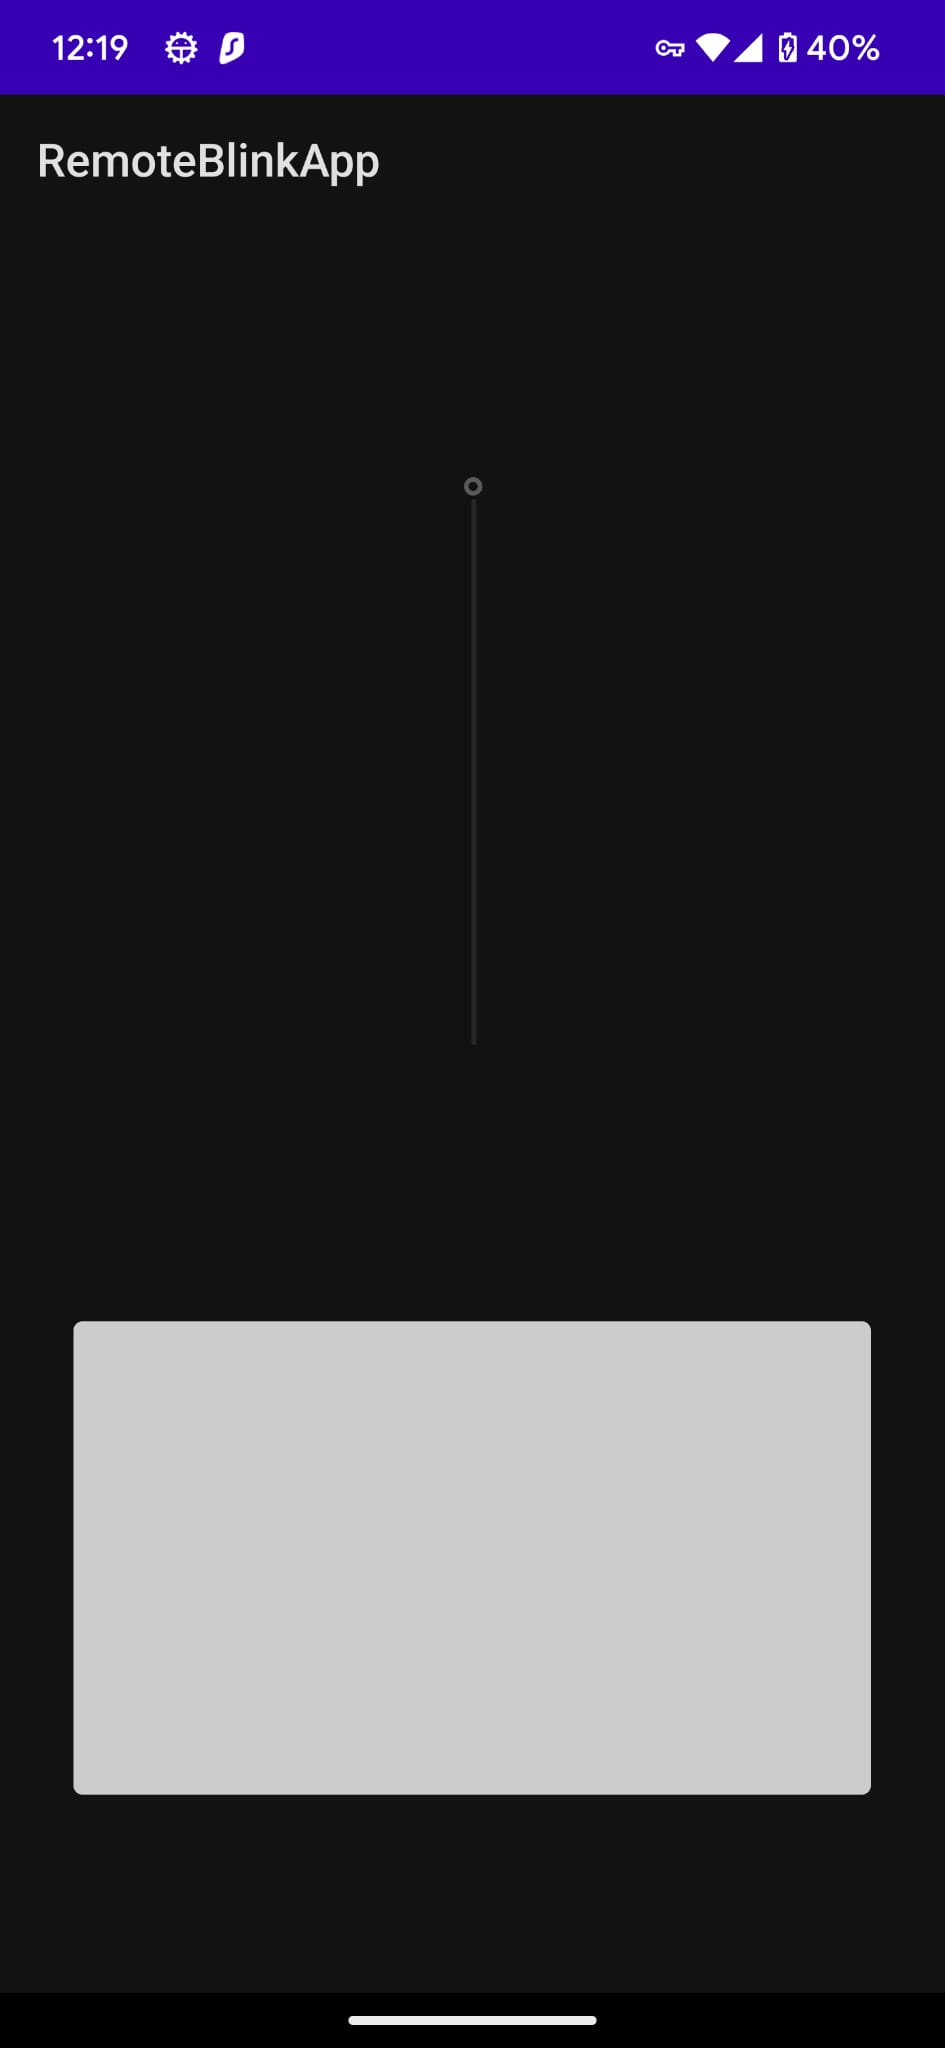
\includegraphics[height=18cm]{mobile-app.jpeg}
    \centering
    \caption{Interfaccia Room App}
\end{figure}

\newpage

% -------------------- Tinkercad --------------------

\section{Tinkercad}

\begin{figure}[H]
    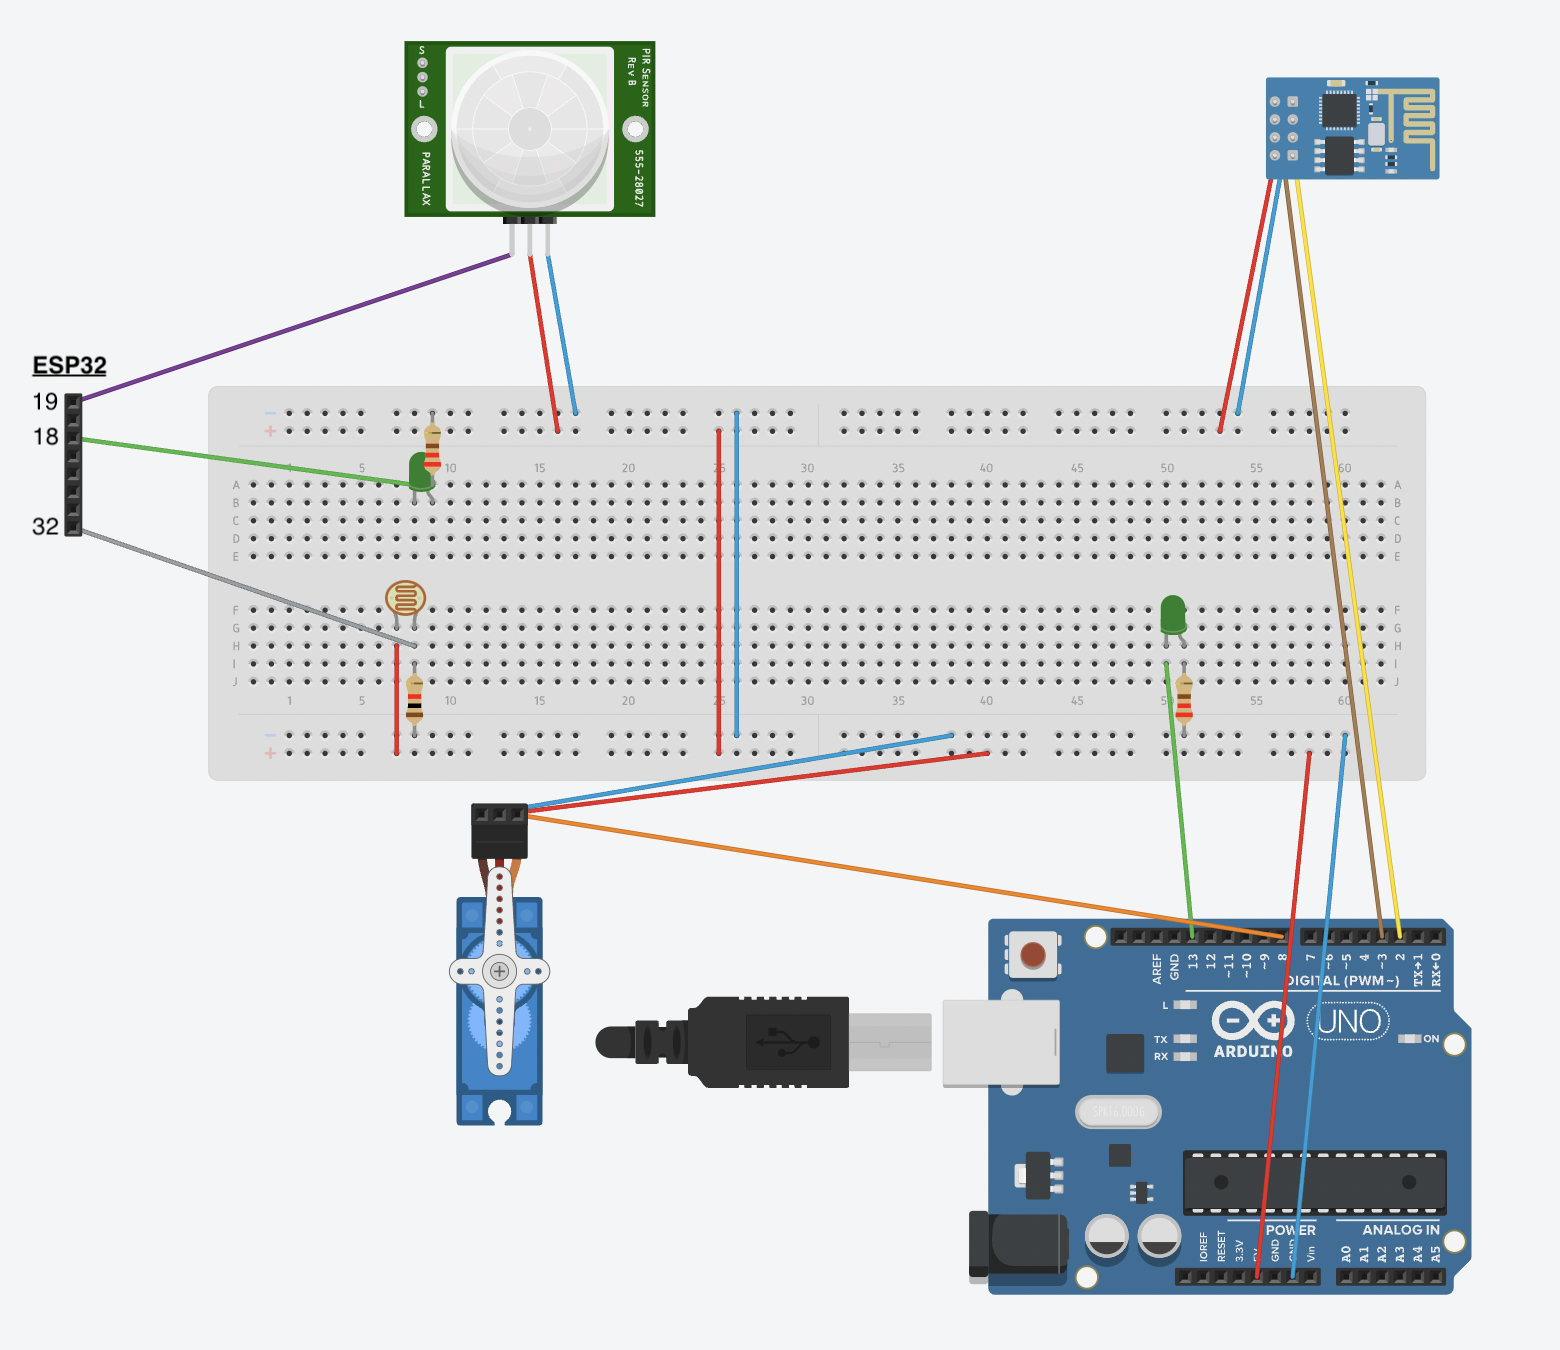
\includegraphics[width=17cm]{tinkercad.png}
\end{figure}

\end{document}